\documentclass[11pt,a4paper]{article}

% --- Core Typography & Geometry ---
\usepackage[utf8]{inputenc}
\usepackage[T1]{fontenc}
\usepackage{lmodern} 
\usepackage[top=0.85in, bottom=0.85in, left=0.85in, right=0.85in]{geometry}
\usepackage{amsmath,amssymb,amsfonts,bm,mathtools}
\usepackage{booktabs,tabularx,array}
\usepackage{graphicx}
\usepackage{caption}
\usepackage{microtype}
\usepackage{enumitem}
\usepackage{titlesec}
\usepackage{xcolor}
\usepackage{fancyhdr}
\usepackage{lastpage}
\usepackage{hyperref}

% --- HKUST Official Palette & Styling ---
\definecolor{hkustnavy}{RGB}{0, 56, 117}
\definecolor{hkustgold}{RGB}{179, 138, 44}
\definecolor{charcoal}{RGB}{35, 35, 35}

\hypersetup{
    colorlinks=true,
    linkcolor=hkustnavy,
    citecolor=hkustnavy,
    urlcolor=hkustnavy
}

% --- Academic Header & Footer Setup ---
\pagestyle{fancy}
\fancyhf{}
\lhead{\footnotesize \textcolor{gray!80!black}{\textsc{HKUST ECON 2123: Macroeconomics} $\cdot$ Problem Set \#1}}
\rhead{\footnotesize \textcolor{gray!80!black}{LIN, Anfan (20861656)}}
\cfoot{\footnotesize \textcolor{gray!80!black}{Page \thepage\ of \pageref{LastPage}}}
\renewcommand{\headrulewidth}{0.4pt}
\renewcommand{\footrulewidth}{0.4pt}

% 首页采用一致的页脚格式
\fancypagestyle{plain}{
    \fancyhf{}
    \renewcommand{\headrulewidth}{0pt}
    \renewcommand{\footrulewidth}{0.4pt}
    \cfoot{\footnotesize \textcolor{gray!80!black}{Page \thepage\ of \pageref{LastPage}}}
}

% --- Section Titles & Spacing ---
\titleformat{\section}{\large\bfseries\color{hkustnavy}}{\thesection}{0.8em}{}[\vspace{-0.3em}\titlerule\vspace{0.2em}]
\titleformat{\subsection}{\normalsize\bfseries\color{black}}{\thesubsection}{0.6em}{}
\titlespacing*{\section}{0pt}{1.0em}{0.35em}
\titlespacing*{\subsection}{0pt}{0.65em}{0.2em}

\setlist[enumerate]{leftmargin=*, label=\arabic*., itemsep=2.5pt, topsep=2pt}
\setlist[itemize]{leftmargin=*, itemsep=2.5pt, topsep=2pt}

\setlength{\parskip}{0.35em}
\setlength{\parindent}{0pt}

\begin{document}

% --- Title Header: Student & Course Meta ---
\begin{flushright}
    \textbf{\large LIN, Anfan (Norman)} \\
    Student ID: \texttt{20861656} \\
    Email: \href{mailto:alinad@connect.ust.hk}{\texttt{alinad@connect.ust.hk}} \\
    BSc in Mathematics (Computer Science Track) \\
    Department of Mathematics, HKUST \\
    \textbf{ECON 2123: Macroeconomics} (Fall 2026) \\
    \today
\end{flushright}

\vspace{-0.6em}
\begin{center}
    {\Large \textbf{\color{hkustnavy}Problem Set \#1: Solutions and Empirical Analysis}} \\
    \vspace{0.25em}
    {\footnotesize \textit{Macroeconomic Measurement, National Accounts Decomposition, Goods Market Equilibrium, and Multipliers}}
\end{center}
\vspace{0.4em}

% =========================================================================
% SECTION 1: REAL GDP AND THE GDP DEFLATOR
% =========================================================================
\section{Real GDP and the GDP Deflator (20 Points)}

\subsection*{(1) Nominal and Real GDP Time Series (10 points)}
Annual macroeconomic data are retrieved from the Census and Statistics Department (C\&SD) of the Hong Kong Special Administrative Region (Table 310-31001: \textit{Gross Domestic Product (GDP), implicit price deflator of GDP and per capita GDP}). We extract ``GDP at current market prices'' (nominal GDP, $Y_t^{\$}$) and ``GDP in chained (2024) dollars'' (real GDP, $Y_t$) for the historical observation window 1961--2025 (65 annual observations). Figure~\ref{fig:gdp_series} plots both series, constructed analogously to Figure 2-1 in Blanchard (2021).

\begin{figure}[htbp]
    \centering
    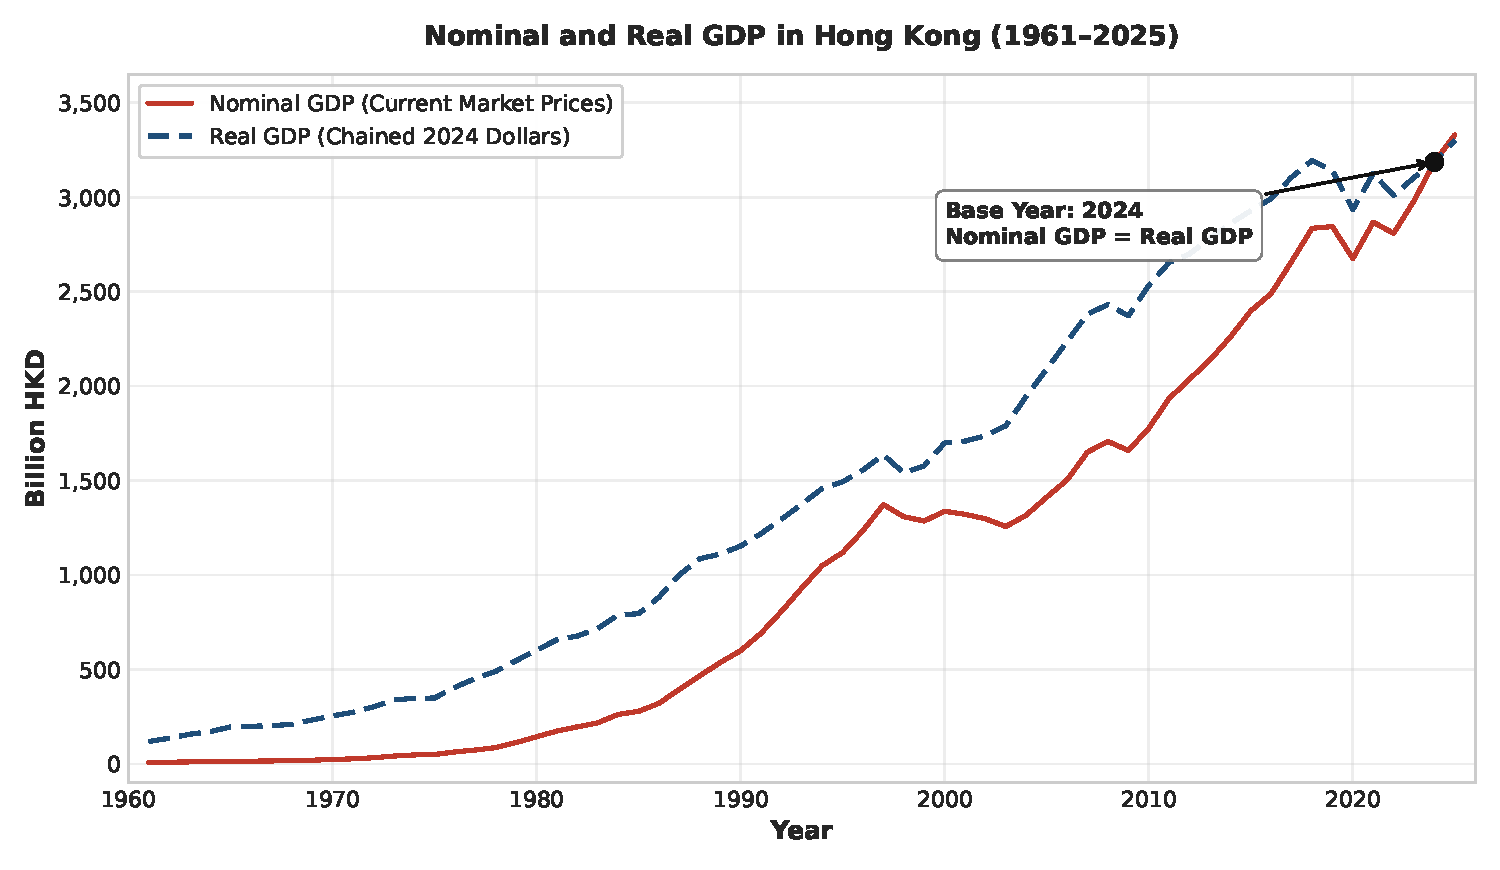
\includegraphics[width=0.76\textwidth]{fig1_nominal_real_gdp}
    \vspace{-0.4em}
    \caption{Nominal and Real GDP in Hong Kong (1961--2025)}
    \label{fig:gdp_series}
    \vspace{-0.3em}
    \begin{minipage}{0.80\textwidth}
        \footnotesize \textit{Data Source:} C\&SD Table 310-31001. Real GDP is expressed in chained (2024) dollars with base year 2024.
    \end{minipage}
\end{figure}

\textbf{Economic and Structural Interpretation:}
\begin{itemize}
    \item \textbf{Base Year Intersection:} The nominal and real GDP curves intersect precisely at the reference base year \textbf{2024}, where $\text{Nominal GDP}_{2024} = \text{Real GDP}_{2024} = \text{HK\$} \, 3,186,526 \text{ million}$, by definition setting the implicit price deflator $P_{2024} \equiv 100$.
    \item \textbf{Pre-2024 Volume Dynamics ($P\_t < 100$):} Prior to 2024, real GDP lies strictly above nominal GDP. Since real GDP measures production using constant base-year (2024) prices:
    \begin{equation*}
        Y_t = \frac{Y_t^{\$}}{P_t / 100}
    \end{equation*}
    Because historical price levels were substantially lower than the 2024 benchmark ($P_t < 100$), dividing by a price index less than 1 scales up the physical volume of production relative to its current-market-price valuation.
    \item \textbf{Post-2024 Trajectory ($P\_t > 100$):} In 2025, nominal GDP (HK\$ 3,329,843 million) exceeds real GDP (HK\$ 3,301,474 million), reflecting cumulative positive price inflation relative to the benchmark year ($P_{2025} = 100.86$).
\end{itemize}

\subsection*{(2) Real GDP Growth Rates and Long-Term Average (5 points)}
For each year $t \in [1962, 2025]$, the annual percentage growth rate of real GDP ($g_{Y, t}$) is given by:
\begin{equation}
    g_{Y, t} = \frac{Y_t - Y_{t-1}}{Y_{t-1}} \times 100\%
\end{equation}
Computing the arithmetic mean across all 64 continuous annual growth rates (identical to Excel's \texttt{AVERAGE} function):
\begin{equation}
    \bar{g}_Y = \frac{1}{64} \sum_{t=1962}^{2025} g_{Y, t} = \mathbf{5.45\%} \quad (5.4468\%)
\end{equation}
\textbf{Macroeconomic Highlights:} Hong Kong exhibited rapid double-digit growth during early export industrialization, peaking at $+16.16\%$ in 1976. Major cyclical troughs reflect severe external shocks: $-5.88\%$ during the 1998 Asian Financial Crisis and an all-time low of $-6.54\%$ during the 2020 pandemic shock.

\subsection*{(3) GDP Deflator and Inflation Rates: Discrete vs. Logarithmic (5 points)}
The implicit GDP deflator ($P_t$, base year $2024 = 100$) and the discrete percentage inflation rate ($\pi_t$) are defined as:
\begin{equation}
    P_t = \frac{\text{Nominal GDP}_t}{\text{Real GDP}_t} \times 100, \qquad \pi_t = \frac{P_t - P_{t-1}}{P_{t-1}} \times 100\%
\end{equation}
Economists also frequently use the natural log-difference to approximate the instantaneous rate of inflation:
\begin{equation}
    \pi_t^{\text{log}} = \Delta \ln P_t \times 100\% = (\ln P_t - \ln P_{t-1}) \times 100\%
\end{equation}
Both series are plotted concurrently in Figure~\ref{fig:inflation_comp}.

\begin{figure}[htbp]
    \centering
    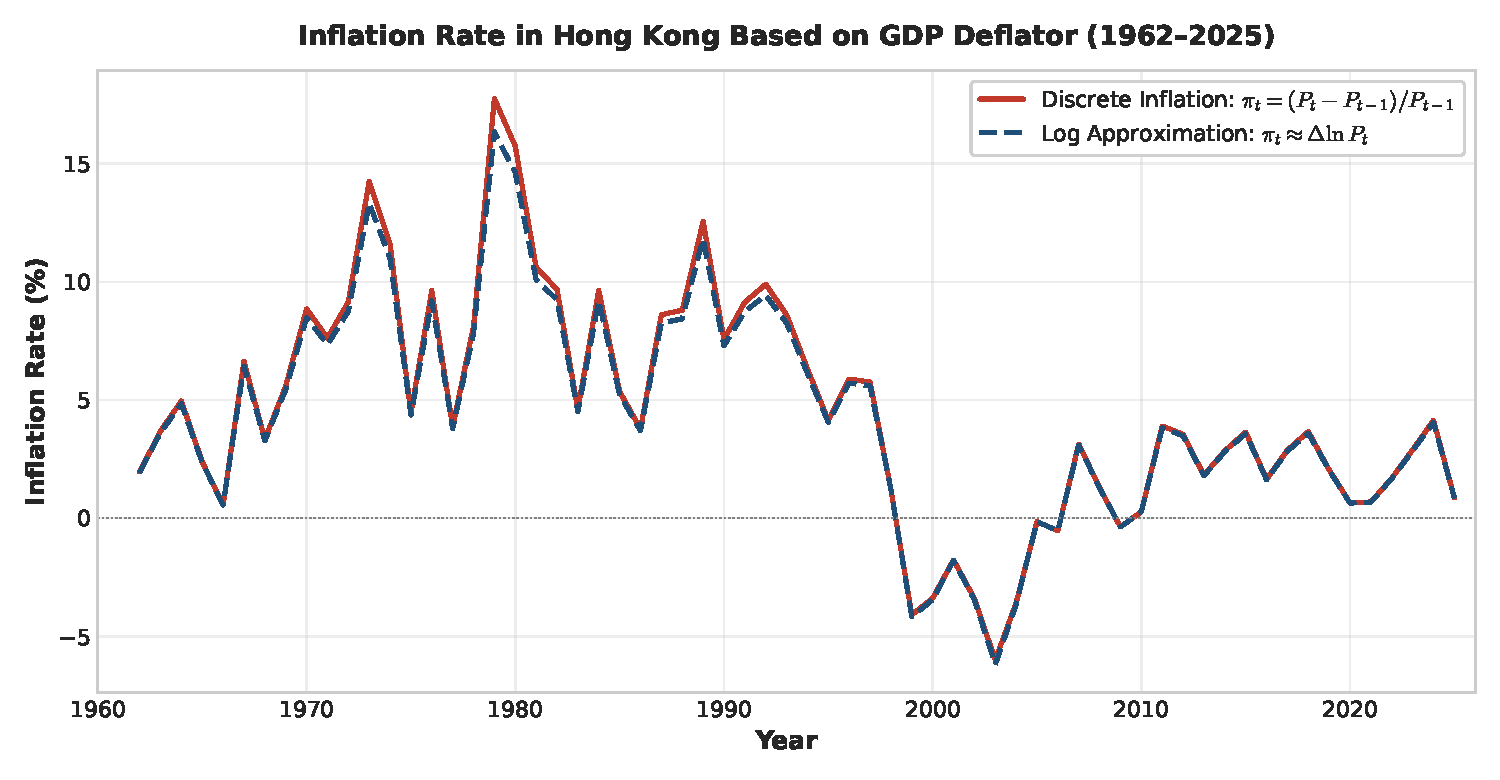
\includegraphics[width=0.76\textwidth]{fig2_inflation_comparison}
    \vspace{-0.4em}
    \caption{Comparison of Discrete and Logarithmic Inflation Rates (1962--2025)}
    \label{fig:inflation_comp}
\end{figure}

\textbf{Mathematical Foundation and Comparative Analysis:}
\begin{itemize}
    \item \textbf{Empirical Similarity:} The two series are almost indistinguishable over the 64-year sample, yielding a Pearson correlation coefficient $\rho = 0.9995$ and an average absolute discrepancy of merely $0.2035\%$.
    \item \textbf{Analytical Justification via Taylor Series:} Factoring the logarithmic difference:
    \begin{equation}
        \Delta \ln P_t = \ln \left( \frac{P_t}{P_{t-1}} \right) = \ln \left( 1 + \frac{P_t - P_{t-1}}{P_{t-1}} \right) = \ln(1 + \pi_t)
    \end{equation}
    Expanding $\ln(1+x)$ via a Maclaurin series for small inflation rates ($\vert{}\pi_t\vert{} \ll 1$):
    \begin{equation}
        \ln(1 + \pi_t) = \pi_t - \frac{1}{2} \pi_t^2 + \frac{1}{3} \pi_t^3 - \cdots = \pi_t - \frac{1}{2}\pi_t^2 + \mathcal{O}(\pi_t^3)
    \end{equation}
    The approximation error is dominated by $\frac{1}{2}\pi_t^2$. When inflation is moderate ($\pi_t \approx 0$), higher-order terms vanish, proving $\Delta \ln P_t \approx \pi_t$.
    \item \textbf{Regime Divergence:} Observable separation occurs strictly in high-inflation regimes. In 1979, discrete inflation peaked at $+17.88\%$ while log-inflation yielded $+16.45\%$ (a $1.43\%$ gap, which closely matches the theoretical second-order penalty $\frac{1}{2}(0.1788)^2 \approx 1.60\%$). Conversely, during low-inflation regimes (e.g., 2015--2025), both measures align. The series also captures Hong Kong's protracted deflationary era from 1998 to 2004 ($\pi_t < 0$, troughing at $-6.18\%$ in 2003).
\end{itemize}

% =========================================================================
% SECTION 2: THE COMPOSITION OF HK GDP, 2023
% =========================================================================
\section{The Composition of HK GDP, 2023 (25 Points)}

\subsection*{(4) Expenditure Components Accounting Table (10 points)}
Using official data from Table 310-31002 (\textit{Gross Domestic Product (GDP) by major expenditure component at current market prices}), the 2023 expenditure components are tabulated in Table~\ref{tab:gdp_composition}. In modern national accounts, total gross investment ($I$) encompasses gross domestic fixed capital formation ($I_{\text{fixed}}$) and changes in inventories ($\Delta \text{Inv}$): $I = I_{\text{fixed}} + \Delta \text{Inv}$.

\begin{table}[htbp]
    \centering
    \small
    \caption{Expenditure Components of Hong Kong GDP (2023, Current Market Prices)}
    \label{tab:gdp_composition}
    \begin{tabularx}{0.92\textwidth}{Xrr}
        \toprule
        \textbf{Component} & \textbf{Millions of HKD, 2023} & \textbf{Percent of GDP (\%)} \\
        \midrule
        \textbf{Gross Domestic Product ($Y$)} & \textbf{2,981,210} & \textbf{100.00\%} \\
        \quad Consumption ($C$) & 2,087,569 & 70.02\% \\
        \quad Investment ($I$) & 481,511 & 16.15\% \\
        \qquad \textit{Gross domestic fixed capital formation} ($I_{\text{fixed}}$) & \textit{505,510} & \textit{16.96\%} \\
        \qquad \textit{Changes in inventories} ($\Delta \text{Inv}$) & \textit{$-$23,999} & \textit{$-$0.81\%} \\
        \quad Government spending ($G$) & 396,813 & 13.31\% \\
        \quad Net Exports ($NX$) & 15,317 & 0.51\% \\
        \qquad Exports of goods and services ($X$) & 5,272,395 & 176.85\% \\
        \qquad Imports of goods and services ($IM$) & 5,257,078 & 176.34\% \\
        \midrule
        Inventory investment ($\Delta \text{Inv}$) & $-$23,999 & $-$0.81\% \\
        \bottomrule
    \end{tabularx}
    \vspace{0.4em}
    \begin{minipage}{0.92\textwidth}
        \footnotesize \textit{National Accounting Identity Balance Check:}
        \begin{align*}
            C + I + G + NX &= 2,087,569 + 481,511 + 396,813 + 15,317 \\
            &= 2,981,210 \equiv Y \quad (\text{Exact closure})
        \end{align*}
    \end{minipage}
\end{table}

\subsection*{(5) Dominant Component of GDP (5 points)}
Among the four primary expenditure components ($C, I, G, NX$), \textbf{Private Consumption Expenditure ($C$)} is the largest component, totaling \textbf{HK\$ 2,087,569 million} and accounting for \textbf{70.02\%} of total GDP in 2023.

\subsection*{(6) Trade Openness Index and US Comparison (5 points)}
From Table 310-31002, the trade and output statistics for Hong Kong in 2022 are:
\begin{align}
    \text{Exports of goods and services } (X_{2022}) &= \text{HK\$} \, 5,463,019 \text{ million} \\
    \text{Imports of goods and services } (IM_{2022}) &= \text{HK\$} \, 5,348,126 \text{ million} \\
    \text{Gross Domestic Product } (Y_{2022}) &= \text{HK\$} \, 2,808,922 \text{ million}
\end{align}
Evaluating the trade openness index:
\begin{equation}
    \text{Openness}_{\mathrm{HK}, 2022} = \frac{X_{2022} + IM_{2022}}{Y_{2022}} = \frac{5,463,019 + 5,348,126}{2,808,922} = \frac{10,811,145}{2,808,922} \approx \mathbf{3.85} \quad (\mathbf{384.89\%})
\end{equation}

\textbf{Economic Comparison with the US Economy ($\approx$25\% in 2023):}
Hong Kong's openness index of $\mathbf{384.89\%}$ is more than \textbf{15 times larger} than that of the United States. This divergence reflects fundamental structural differences:
\begin{enumerate}
    \item \textbf{Global Entrep\^ot and Re-export Intermediation:} Hong Kong operates as an ultra-open international trading and logistics hub. Trade statistics reflect gross commercial turnover ($X, IM$), whereas GDP measures net domestic value-added ($Y$). Intermediate merchandise and re-exports moving through Hong Kong routinely exceed domestic economic value-added multiple times over.
    \item \textbf{Continental Economy vs. Small Open Economy:} The US is a continental-scale, highly self-sufficient economy where interstate domestic trade forms the core economic engine; cross-border international trade naturally constitutes a modest fraction of aggregate GDP.
\end{enumerate}

\subsection*{(7) Industry-Wise Decomposition (5 points)}
From Table 310-34101 (\textit{Gross Domestic Product (GDP) by major economic activity - percentage contribution to GDP}), the contributions of the five primary economic sectors in 2023 are:
\begin{enumerate}
    \item Agriculture, fishing, mining and quarrying: $0.0\%$
    \item Manufacturing: $1.0\%$
    \item Electricity, gas and water supply, and waste management: $1.1\%$
    \item Construction: $4.3\%$
    \item \textbf{Services}: $\mathbf{93.5\%}$
\end{enumerate}
The overwhelmingly dominant industry is \textbf{Services}, accounting for \textbf{93.5\%} of Hong Kong's GDP in 2023. Key drivers include Financing and Insurance ($24.9\%$) alongside Import/Export, Wholesale and Retail Trades ($17.5\%$).

% =========================================================================
% SECTION 3: THE EMPLOYMENT RATE
% =========================================================================
\section{The Employment Rate (10 Points)}

\subsection*{(8) Derivation of the Employment Rate (10 points)}
Let the macroeconomic labor aggregates be defined as:
\begin{itemize}
    \item $\text{WAP}$: Working-Age Population
    \item $L$: Labor Force, where $L = E + U$ ($E$: Employed, $U$: Unemployed)
\end{itemize}
Following standard OECD definitions:
\begin{align}
    \text{Participation Rate } (PR) &\equiv \frac{L}{\text{WAP}} = 0.80 \\
    \text{Unemployment Rate } (u) &\equiv \frac{U}{L} = \frac{L - E}{L} = 1 - \frac{E}{L} = 0.10 \implies \frac{E}{L} = 1 - u = 0.90 \\
    \text{Employment Rate } (ER) &\equiv \frac{E}{\text{WAP}}
\end{align}
Factoring the employment rate definition into the product of labor participation and employment intensity:
\begin{equation}
    ER = \frac{E}{\text{WAP}} = \left( \frac{E}{L} \right) \times \left( \frac{L}{\text{WAP}} \right) = (1 - u) \times PR
\end{equation}
Substituting the parameter values:
\begin{equation}
    ER = (1 - 0.10) \times 0.80 = 0.90 \times 0.80 = \mathbf{0.72} \quad (\mathbf{72.0\%})
\end{equation}
The employment rate in this economy is \textbf{72\%}. Note that $ER \neq 1 - u$ because the denominator of the unemployment rate is the active labor force ($L$), whereas the denominator of the employment rate is the total working-age population ($\text{WAP}$).

% =========================================================================
% SECTION 4: GOODS MARKET EQUILIBRIUM & MULTIPLIERS
% =========================================================================
\section{Goods Market Equilibrium and Multipliers (55 Points)}

Consider the following goods market system for a closed economy (in billions of euros):
\begin{equation}
    C = 480 + 0.5 Y_D, \quad I = 110, \quad T = 70, \quad G = 250, \quad Y_D \equiv Y - T
\end{equation}

\subsection*{(9) Goods Market Equilibrium Output ($Y^*$) (10 points)}
In equilibrium, aggregate output equals aggregate demand ($Y = Z$):
\begin{align}
    Y &= C + I + G = [480 + 0.5(Y - 70)] + 110 + 250 \\
    Y &= 480 + 0.5Y - 35 + 110 + 250 = 805 + 0.5Y \\
    (1 - 0.5) Y &= 805 \implies 0.5 Y = 805 \implies Y^* = \frac{805}{0.5} = \mathbf{1,610} \text{ billion euros}
\end{align}

\subsection*{(10) Equilibrium Disposable Income ($Y_D^*$) (5 points)}
\begin{equation}
    Y_D^* = Y^* - T = 1,610 - 70 = \mathbf{1,540} \text{ billion euros}
\end{equation}

\subsection*{(11) Equilibrium Consumption ($C^*$) (5 points)}
\begin{equation}
    C^* = 480 + 0.5(1,540) = 480 + 770 = \mathbf{1,250} \text{ billion euros}
\end{equation}
\textit{Goods Market Clearing Verification:}
\[Z^* = C^* + I + G = 1,250 + 110 + 250 = 1,610 \equiv Y^*\]

\subsection*{(12) Savings and Investment Accounting (5 points)}
\begin{itemize}
    \item \textbf{Private Savings ($S\_{\text{private}}$):}
    \begin{equation}
        S_{\text{private}} = Y_D^* - C^* = 1,540 - 1,250 = \mathbf{290} \text{ billion euros}
    \end{equation}
    Equivalently, via the private savings function:
    \begin{equation}
        S_{\text{private}} = -c_0 + (1 - c_1)Y_D = -480 + (1 - 0.5)(1,540) = -480 + 770 = 290
    \end{equation}
    \item \textbf{Public Savings ($S\_{\text{public}}$):}
    \begin{equation}
        S_{\text{public}} = T - G = 70 - 250 = \mathbf{-180} \text{ billion euros} \quad (\text{Budget Deficit of 180})
    \end{equation}
    \item \textbf{Investment Spending ($I$):}
    \begin{equation}
        I = \mathbf{110} \text{ billion euros}
    \end{equation}
\end{itemize}
\textbf{IS Identity Check:} Total national savings equals investment:
\[S_{\text{total}} = S_{\text{private}} + S_{\text{public}} = 290 + (-180) = 110 \equiv I\]

\subsection*{(13) Government Spending Multiplier ($\Delta Y / \Delta G$) (5 points)}
Holding taxes fixed ($\Delta T = 0$):
\begin{equation}
    \frac{\Delta Y}{\Delta G} = \frac{1}{1 - c_1} = \frac{1}{1 - 0.5} = \frac{1}{0.5} = \mathbf{2}
\end{equation}
A one-unit expansion in government spending increases equilibrium output by \textbf{2 units}.

\subsection*{(14) Tax Multiplier ($\Delta Y / \Delta T$) (5 points)}
Holding government spending fixed ($\Delta G = 0$):
\begin{equation}
    \frac{\Delta Y}{\Delta T} = \frac{-c_1}{1 - c_1} = \frac{-0.5}{1 - 0.5} = \frac{-0.5}{0.5} = \mathbf{-1}
\end{equation}
A one-unit increase in lump-sum taxes contracts equilibrium output by \textbf{1 unit}.

\subsection*{(15) Balanced Budget Multiplier ($\left. \Delta Y / \Delta G \right\vert{}_{\Delta G = \Delta T}$) (5 points)}
Under a balanced budget fiscal expansion where $\Delta G = \Delta T$:
\begin{equation}
    \left. \frac{\Delta Y}{\Delta G} \right|_{\Delta G = \Delta T} = \frac{\Delta Y}{\Delta G} + \frac{\Delta Y}{\Delta T} = \frac{1}{1 - c_1} + \frac{-c_1}{1 - c_1} = \frac{1 - c_1}{1 - c_1} = \mathbf{1}
\end{equation}
Output expands dollar-for-dollar with government purchases (Haavelmo's theorem), because government spending stimulates aggregate demand directly, whereas households absorb part of the tax hike by reducing private savings.

\subsection*{(16) Income-Dependent Taxes and Recalculated Multiplier (10 points)}
Suppose taxes depend endogenously on aggregate income:
\begin{equation}
    T = t_0 + t_1 Y = -252 + 0.2 Y, \quad \text{where } t_0 = -252, \; t_1 = 0.2
\end{equation}
Substituting this tax rule into aggregate demand:
\begin{align}
    Y &= c_0 + c_1[Y - (-252 + 0.2Y)] + I + G \\
    Y &= c_0 + c_1(1 - 0.2)Y - c_1(-252) + I + G \\
    [1 - c_1(1 - t_1)] Y &= [c_0 - c_1 t_0 + I + G] \implies Y = \frac{c_0 - c_1 t_0 + I + G}{1 - c_1(1 - t_1)}
\end{align}
Differentiating with respect to $G$:
\begin{equation}
    \frac{\Delta Y}{\Delta G} = \frac{1}{1 - c_1(1 - t_1)} = \frac{1}{1 - 0.5(1 - 0.2)} = \frac{1}{1 - 0.4} = \frac{1}{0.6} = \mathbf{\frac{5}{3}} \approx \mathbf{1.67}
\end{equation}
The government spending multiplier falls from $2.00$ to $\mathbf{1.67}$ (or $5/3$).

\textit{Remark on Baseline Equilibrium:} At the original equilibrium $Y^* = 1,610$, endogenous tax collection equals $T = -252 + 0.2(1,610) = 70$. Thus, baseline equilibrium output is preserved at $1,610$, but output responsiveness to exogenous shocks is substantially stabilized.

\subsection*{(17) Macroeconomic Rationale for Automatic Stabilizers (5 points)}
An income-dependent tax system functions as an \textbf{automatic stabilizer} through two mechanisms:
\begin{enumerate}
    \item \textbf{Built-in Cushioning of Disposable Income:} When an adverse shock reduces aggregate output ($\Delta Y < 0$), tax revenue automatically declines by $\Delta T = t_1 \Delta Y < 0$. Disposable income falls by only $\Delta Y_D = (1 - t_1) \Delta Y$, ensuring that $\vert{}\Delta Y_D\vert{} < \vert{}\Delta Y\vert{}$. Consequently, private consumption declines less severely than it would under lump-sum taxes.
    \item \textbf{Damping of Multiplier Dynamics without Policy Lag:} The expenditure multiplier is lowered from $\frac{1}{1-c_1} = 2.0$ to $\frac{1}{1-c_1(1-t_1)} \approx 1.67$. Because this damping operates endogenously and instantaneously without administrative, legislative, or implementation lags, it reduces business cycle volatility.
\end{enumerate}

\end{document}